%\usepackage{amsmath} %<-- ajaja quien puso esto aca??
\section{Ejercicio 2}

\subsection{Interpretación del enunciado}
\par{Se tienen una cantidad $n$ de cursos con sus respectivas fechas de inicio y finalizaci\'on representadas con n\'umeros enteros positivos. El objetivo de este ejercicio es desarrollar un algoritmo que, dadas las fechas de inicio y fin de cada curso, encuentre un subconjunto de cursos que no se solapen entre s\'i, es decir, sean compatibles. Se pide que la complejidad del algoritmo sea estrictamente menor a O($n$^{2})$ siendo $n$ la cantidad de cursos$.}
\par{Para este ejercicio, asumiremos que los cursos no se interrumpen. Es decir, por ejemplo, que el curso que arranca el día 5 y termina el día 8 va a dictarse también los días 6 y 7. Entonces lo que nos queda es un problema de optimización: ¿Cómo elegir la mayor cantidad de cursos posibles de manera que ningún par de cursos dado tenga días en común?. En particular para que se puedan tomar dos cursos, la fecha de inicio de uno de los dos tiene que ser mayor (estricto) que la fecha de finalizacon del otro curso.}
\par{Cabe destacar que lo que este problema busca es maximizar la cantidad de cursos disponibles para ser cursados por un único alumno, y no buscar que haya más días cubiertos por un curso. También hay que mencionar que los cursos no tienen ningún valor numérico asignado.}
%	PONER EJEMPLOS

\subsection{Resolución}
\par{Para resolver este ejercicio se desarroll\'o un algoritmo goloso. Se busca devolver un conjunto de cursos. El algoritmo itera agregando, en caso de ser posible, un curso en cada iteraci\'on. Mientras se pueda seguir agregando cursos (no se puede si todos los restantes se solapan con alguno seleccionado), se agrega de los que quedan, el de menor fecha de finalizaci\'on que no se solape con alguno seleccionado. Luego se devuelven los cursos seleccionados.}
\par{A continuación expondremos un pseudocódigo de la solución implementada. Suponemos los datos levantados directamente desde la entrada y almacenados en un vector de cursos llamado $cronograma$.}\

%~ \begin{algorithm}[H]
%~ \SetLine
%~ \hspace{-13pt}\textbf{cronograma} resolver(\textbf{cronograma} $C$)\\
%~ C $\longleftarrow$ ordenar$\_$finalización($C$)\\
%~ $ultimaFecha \longleftarrow -1$\\
%~ $cronograma\_aceptado \longleftarrow \emptyset$\\
%~ \ForEach{c $\in$ C}{
  %~ \If{$fechaInicio(c) > ultimaFecha$}{
        %~ $cronograma\_aceptado \longleftarrow cronograma\_aceptado \cup c$\\
        %~ $ultimaFecha \longleftarrow fechaFin(c)$\\
  %~ }
%~ }
%~ \textbf{return} $cronograma\_aceptado$\\
%~ \caption{Resolución Golosa Ejercicio 2}
%~ \end{algorithm}
%~ 
\begin{algorithm}[H]
	\caption{Resolución Golosa Ejercicio 2}
	\begin{algorithmic}
		\KwData{vector(Curso) $entrada$}\\
		vector(Curso) $cronograma\_aceptado \longleftarrow \emptyset$\\
		\While{$puedoAgregarCursos$}{ 
			$cronograma\_aceptado \longleftarrow cronograma\_aceptado$ \cup\\
			$c \in entrada$ / $sonCompatibles(c, cronograma\_aceptado)$ \land \\
							$fechaFin(c) \geq fechaFin(c')$ \forall c'$ \in$ $entrada$
		}
		\textbf{return} $cronograma\_aceptado$\\
	\end{algorithmic}
\end{algorithm}
\par{El vector de cursos $entrada$ contiene todos los cursos de la instancia, mientras que el vector $cronograma\_aceptado$ contiene los que se van agregando a la soluci\'on. La funci\'on $sonCompatibles$ devuelve si el curso $c$ no se solapa con alg\'un curso del vector de aceptados.}

%~ \subsection{Complejidad}
%~ En lo que a complejidad se refiere, los fragmentos más costosos de nuestro algoritmo son la función ordenar$\_$finalización (l.2) y el ciclo que recorre linealmente todos los cursos $c$ dentro del cronograma $C$ (l.5). La función ordenar$\_$finalización está implementada mediante la función \textfff{sort} dentro de la STL de \textfff{C++}. La misma tiene una complejidad de $O(n log n)$ \footnote{http://www.cplusplus.com/reference/algorithm/sort/}. El ciclo de que recorre todos los cursos del cronograma $C$ tiene una complejidad de $O(n)$, ya que implementamos el cronograma sobre un vector. Luego, la complejidad de nuestra función resolver termina siendo de $T(n) = O(n log n) + O(n) = O(n log n)$.

\subsection{Complejidad}
\par{Para obtener en cada iteraci\'on del ciclo principal (l\'inea 2) el curso con menor fecha de finalizaci\'on, se pueden ordenar, antes de entrar al ciclo, los cursos seg\'un su fecha de finalizaci\'on. Ordenar los cursos puede hacerse en $O(n log n)$ con $n$ la cantidad de elementos a ordenar, en este caso, la cantidad de cursos de la entrada. Luego, con los cursos ordenados, el ciclo debe iterar sobre los $n$ cursos, evaluando si cada uno es compatible con el resto del cronograma aceptado. Esto puede hacerse determinando si se solapa con el anterior (como se agregan en orden, si se solapa con alguno, tiene que ser con el \'ultimo agregado), lo cual tiene complejidad O(1), ya que es una comparaci\'on de enteros (la fecha de finalizaci\'on del curso que se itera y la del \'ultimo curso agregado). Entonces, El ciclo que recorre los $n$ cursos del cronograma de entrada tiene una complejidad de $O(n)$. Luego, la complejidad de la función $resolver$ termina siendo de $T(n) = O(n log n) + O(n) = O(n log n)$.}

\subsection{Implementaci\'on}
\par{La implementaci\'on de este algoritmo en C++ primero ordena los cursos seg\'un su fecha de finalizaci\'on. Luego recorre todos los cursos en orden y para cada curso, eval\'ua si puede ser agregado o no. La función de ordenamiento está implementada mediante la función \textfff{sort} dentro de la STL de \textfff{C++}. La misma tiene una complejidad de $O(n log n)$ \footnote{http://www.cplusplus.com/reference/algorithm/sort/}. En cada iteraci\'on del ciclo que recorre los cursos, no hace m\'as que comparar la fecha de finalizaci\'on del curso que se itera con la del \'ultimo curso agregado. Si es mayor estricta, agrega el curso a los cursos aceptados.}

\subsection{Demostraci\'on de Correctitud}
\par{En esta secci\'on vamos a demostrar que el algoritmo resuelve el problema de encontrar la m\'axima cantidad de cursos que no se superponen.
Para eso demostraremos las siguientes propiedades:}

\begin{itemize}
\item \textbf{Prop 1: }\emph{Sea B un conjunto de cursos que maximiza la cantidad de cursos compatibles, y sea A el conjunto que siempre elige la de menor fecha de finalizaci\'on que sea compatible, \#A = \#B.}
\item \textbf{Prop 2: }\emph{Nuestro algoritmo siempre elige la de menor fecha de finalizaci\'on que sea compatible.}\\
\end{itemize}

%\textbf{1. Sea B un conjunto de cursos que maximiza la cantidad de cursos compatibles,
%   y sea A el conjunto que siempre elige la de menor fecha de finalizaci\'on que sea compatible. Luego \#A = \#B.}\\
%Para esto veremos que una solucion al problema reside en tomar el curso de menor fecha de finalizacion que sea compatible con
%los cursos tomados hasta el momento de la seleccion y encontrar la maxima cantidad de cursos que sean compatibles con el curso que acabamos de elegir.

\textbf{Prop 1)} Para demostrar esto, emplearemos la siguiente notaci\'on: Sea A = $\{A_1,A_2,A_3...A_k\}$ el conjunto de cursos que da nuestro algoritmo, donde se cumple que:
\begin{equation}
fechaFin(A_i)<fechaFin(A_j) \quad \forall i\textlessj ,1\le i<j\le k\\
\end{equation}
con $k$ la cantidad de cursos de nuestra soluci\'on; y definiendo a B = $\{B_1,B_2,B_3..B_m\}$, donde:\\
\begin{equation}
fechaFin(Ai)\textless fechaFin(A_j) \quad \forall i<j, 1\le i<j\le m\\ 
\end{equation}
con $m$ la cantidad de cursos de la soluci\'on \'optima, como B es el conjunto de cursos de la soluci\'on \'optima vale que $k\le m$ .\\

\textbf{Lema:} $FechaFin(A_i) \le FechaFin(B_i)$ $\forall i: 1\le i \le k$. Probaremos esto por inducción. Queremos ver que:
\begin{equation}
	fechaFin(A_i)\leq fechaFin(B_i) \quad \forall i: 1\le i \le k 
\end{equation}

Tomamos como caso base $fechaFin(A_1)\leq fechaFin(B_1)$. Esto es cierto ya que al inicio del algoritmo, cualquier curso es compatible (ya que el conjunto de cursos seleccionados hasta ese momento es vac\'io) y adem\'as el algoritmo siempre selecciona el curso compatible con menor fecha de finalizaci\'on. Luego queda probado el caso base.\\

Nuestro paso inductivo requiere probar que:
\begin{equation}
\forall c : 1 \le c < k \quad fechaFin(A_c)\leq fechaFin(B_c) \quad \Rightarrow fechaFin(A_{c+1})\leq fechaFin(B_{c+1})
\end{equation}

Como vale la hip\'otesis inductiva sabemos que $fechaFin(A_c)\leq fechaFin(B_c)$. Tambi\'en sabemos que la $fechaFin(B_{c+1}) > fechaInicio(B_{c+1})$ y, como B es un conjunto que tiene a cursos compatibles tenemos que $fechaInicio(B_{c+1}) > fechaFin(B_c)$. Luego con la afirmaci\'on anterior sumada a la hip\'otesis inductiva podr\'iamos seleccionar el curso $B_{c+1}$:

	  \begin{equation}
		fechaFin(A_c) \stackrel{\rm{por HI}} \le  fechaFin(B_c) \stackrel{\rm{B conj compatible}} < fechaInicio(B_{c+1})   \\ 
	\end{equation}
	  \\ Ya que nuestro algoritmo selecciona el curso compatible con menor fecha de finalización, se deduce
	  que $fechaFin(A_{c+1})\le fechaFin(B_{c+1})$ \Box \\
	  
	
Con el lema podremos probar que vale que $k\ge m$, y como sab\'iamos que $k\le m$ tendremos que el conjunto
de soluciones dadas por el algoritmo es \'optimo en cuanto a maximizar la cantidad de cursos que sean compatibles. Demostraremos, a continuación, que $K\ge m$, por el absurdo.\\ 

Sea $B$ el conjunto que maximiza la cantidad de cursos con un cardinal de $m$, y el conjunto que devuelve nuestro algoritmo un cardinal de $k$. Supongamos que $k<m$ y lleguemos a un absurdo.
Como $B$ es un conjunto que tiene cursos compatibles, el curso $B_{k+1}$ es compatible con el conjunto $\{B_1,B_2,B_3..B_k\}$. Del lema sabemos que $FechaFin(A_k) \le fechaFin(B_k)$, por lo tanto $B_{k+1}$ tambi\'en ser\'ia compatible con el conjunto $\{A_1,A_2,A_3..A_k\}$. Luego, ese curso entraria en el cronograma de cursos acepatados de nuestro algoritmo. Esto es un absurdo, ya que supusimos que $\#A = k$ \Box\\


\textbf{Prop 2)} Es preciso notar que nuestro algoritmo ordena en forma creciente de acuerdo a la fecha de finalizaci\'on y luego recorre desde el de menor fecha, hasta el de mayor fecha de finalizaci\'on. Por otro lado siempre elige tomar un curso m\'as, si este es compatible ya que de la forma que recorremos vale que:
\begin{equation}
fechaFin(curso_{iteracionj}) \geq fechaFin(curso_{iteracioni}) \quad \forall j>i
\end{equation}


Adem\'as el algoritmo en cada iteraci\'on comprueba que: 
\begin{equation}
fechaInicio(curso_{iteracionj}) > ultimaFechaFin 
\end{equation}
para que no haya solapamientos entre el curso a elegir con los ya elegidos anteriormente.\\
Esto es v\'alido debido a que la $fechaInicio(curso_{iteracionj}) > ultimaFechaFin $ y\\
$fechaFin(curso_{iteracionj}) \geq fechaFin(curso_{iteracioni}) \quad \forall j>i$\\

\newpage
\subsection{Testing}
\textbf{Correctitud}\\
Los tests expuestos a continuación fueron diseñados con el fin de verificar diferentes casos particulares que pudimos identificar. Para cada test vamos a exponer la entrada, la salida y, en caso de que sea necesario, una justificaci\'on de la correctitud de la soluci\'on.\\

\noindent\textbf{Test$\#$1}\\
\textbf{Caracterización:} Varios cursos que no coinciden en ningún dia.\\
\textbf{Input:} \textfff{4 1 2 3 4 5 6 7 8}\\
\textbf{Output:} \textfff{1 2 3 4}\\
\textbf{Status:} OK. Los 4 cursos se pueden tomar.\\

\noindent\textbf{Test$\#$2}\\
\textbf{Caracterización:} Varios cursos, todos incompatibles entre si.\\
\textbf{Input:} \textfff{3 1 5 2 6 3 7}\\
\textbf{Output:} \textfff{1}\\
\textbf{Status:} OK. Si bien elegir cualquiera de los cursos es solución, nuestro algorimo elije el primero analizado.\\

\noindent\textbf{Test$\#$3}\\
\textbf{Caracterización:} Prioriza obtener la mayor cantidad de cursos, por sobre la mayor cantidad de horas cursadas.\\
\textbf{Input:} \textfff{4 9 15 3 7 21 27 1 31}\\
\textbf{Output:} \textfff{2 1 3}\\
\textbf{Status:} OK. Se descarta el curso que dura desde el 1ro hasta el 31 del mes, para que se puedan dictar los 3 cursos que no se solapan entre si.\\

\noindent\textbf{Test$\#$4}\\
\textbf{Caracterización:} Cursos encadenados.\\
\textbf{Input:} \textfff{11 1 2 2 3 3 4 4 5 5 6 6 7 7 8 8 9 9 10 10 11 11 12}\\
\textbf{Output:} \textfff{1 3 5 7 9 11}\\
\textbf{Status:} OK. Se preserva la mayor cantidad de cursos, eliminando los necesarios para ``desconectar'' toda la serie. En estos casos, hay que eliminar un curso de por medio.\\

\newpage
\textbf{Performance}\\
\par{Para realizar los tests de performance escribimos un programa (\textfff{testGen.cpp}) que genera de manera aleatoria varias instancias de prueba para cada $n$ entre 1 y 1000000 con un salto de 10000(20 mediciones por cada n). Para poder visualizar de la mejor manera posible la curva de performance de nuestro programa, programamos nuestro generador para que produzca tests en el peor caso posible\footnote{Las mediciones de tiempos de las instancias se encuentran en codigo/ej2/tests/test.out}. Para ese ejercicio, y viendo que la complejidad de nuestro algoritmo viene dada por la operación de ordenamiento, decidimos generar los tests de modo tal que las fechas de inicializacion y finalizacion de cada curso sea aleatoria. En el gráfico agregamos la función $f = C * n log (n)$ donde C = $\frac{1}{37500000}$ } que acota por arriba a la media de las mediciones.

\begin{figure}[H]
\centering
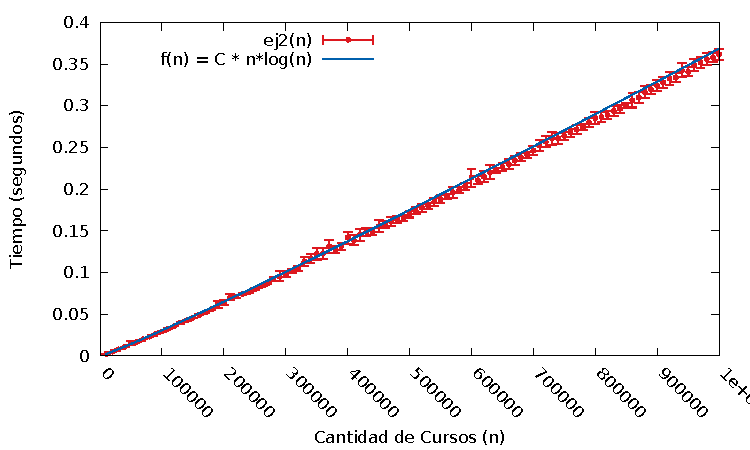
\includegraphics{imgs/ej2.pdf}
\caption{Test de Performance: Tiempo(s) vs Cantidad de Cursos}
\end{figure}

